\documentclass[12pt, a4paper]{article}
\usepackage[utf8]{inputenc}
\usepackage[T2A]{fontenc}
\usepackage[russian]{babel}
\usepackage[top=2cm, bottom=2cm, left=2.5cm, right=1.5cm]{geometry}
\usepackage{listings}
\usepackage{xcolor}
\usepackage{graphicx}
\usepackage{hyperref}
\usepackage{indentfirst}
\usepackage{setspace}
\usepackage{listings}
\usepackage{xcolor}
\usepackage{listingsutf8} % add this in preamble
\usepackage{minted} % put in preamble

% --- SQL listing style ---
\lstdefinestyle{sql}{
    language=SQL,
    basicstyle=\ttfamily\small,
    keywordstyle=\bfseries\color{blue!70!black},
    commentstyle=\itshape\color{gray},
    stringstyle=\color{red!60!black},
    breaklines=true,
    breakatwhitespace=true,
    frame=single,
    numbers=none,
    showstringspaces=false,
    tabsize=2,
    morekeywords={SERIAL, VARCHAR, BOOLEAN, TIMESTAMPTZ, DOMAIN, TYPE,
                  ENUM, POINT, GENERATED, ALWAYS, STORED, uint2, BEGIN,
                  COMMIT, CREATE, INSERT, INTO, VALUES, REFERENCES,
                  PRIMARY, KEY, CONSTRAINT, NOT, NULL, DEFAULT, CHECK,
                  AS, AND, INT, INT4, TIME, DATE, INDEX, ON, UNIQUE,
                  DELETE, UPDATE, CASCADE, CURRENT_DATE, TRIM, INTEGER}
}

\begin{document}

% ========== TITLE PAGE ==========
\begin{titlepage}
    \centering
    \textbf{Санкт-Петербургский Национальный Исследовательский Университет ИТМО}\\
    \textbf{Факультет Программной Инженерии и Компьютерной Техники}

    \vspace{2cm}
    
\includegraphics[width=0.4\textwidth]{ITMOLogo.png}\\[1cm]

    \vspace{3cm}
    {\Large Вариант №473397\\[0.4em]
    Лабораторная работа №1\\[0.4em]
    По дисциплине Базы Данных\\[0.4em]
    }

    \vfill
    \begin{flushright}
        Выполнил студент:\\
        Эллити Мохамед Эмад Ахмед Авад\\[1em]
        Группы:\\ P3131 \\[1em]
        Преподаватель:\\
        Коновалов Арсений Антонович\\
        Николаев Владимир Вячеславович
    \end{flushright}

    \vspace{2cm}
    Санкт-Петербург 2026 г.
\end{titlepage}

% ========== SECTION 1 ==========
\section{Текст задания}

Для выполнения лабораторной работы №1 необходимо:

\begin{enumerate}
    \item На основе предложенной предметной области (текста) составить её описание. Из полученного описания выделить сущности, их атрибуты и связи.
    \item Составить инфологическую модель.
    \item Составить даталогическую модель. При описании типов данных для атрибутов должны использоваться типы из СУБД PostgreSQL.
    \item Реализовать даталогическую модель в PostgreSQL. При описании и реализации даталогической модели должны учитываться ограничения целостности, которые характерны для полученной предметной области.
    \item Заполнить созданные таблицы тестовыми данными.
\end{enumerate}

% ========== SECTION 2 ==========
\section{Описание предметной области}

Описание предметной области, по которой должна быть построена доменная модель:

\begin{quote}
Олвин слегка поклонился в знак признательности, огромные двери снова раздвинулись перед ним, и он медленно вышел из зала. Джизирак последовал за ним и, когда створки дверей снова сомкнулись, повернулся к своему воспитаннику.
\end{quote}

Человек находится в зале. В зале есть огромные двери, которые могут быть открыты или закрыты. Джизирак~--- наставник Олвина. Олвин~--- его воспитанник.
\newpage
% ========== SECTION 3 ==========
\section{Список сущностей и их классификация}

\textbf{Стержневые:}
\begin{itemize}
    \item \textbf{Персонаж (Person)} --- уникальный идентификатор (\texttt{person\_id}), имя (\texttt{name}).
    \item \textbf{Зал (Hall)} --- идентификатор (\texttt{hall\_id}), название (\texttt{name}), тип (\texttt{type}), кампус (\texttt{campus\_id}).
    \item \textbf{Кампус (Campus)} --- идентификатор (\texttt{campus\_id}), название (\texttt{name}).
    \item \textbf{Предмет (Subject)} --- идентификатор (\texttt{subject\_id}), название (\texttt{name}).
\end{itemize}

\textbf{Характеристические:}
\begin{itemize}
    \item \textbf{Дверь (Door)} --- идентификатор (\texttt{door\_id}), размер (\texttt{size}, например «огромные»), состояние (\texttt{state}: «open» или «closed»), зал (\texttt{hall\_id}).
\end{itemize}

\textbf{Ассоциативные:}
\begin{itemize}
    \item \textbf{Наставничество (Mentorship)} --- идентификатор (\texttt{mentorship\_id}), наставник (\texttt{mentor\_id}), воспитанник (\texttt{ward\_id}), дата начала (\texttt{start\_date}).
    \item \textbf{Преподавание (Teaching)} --- идентификатор (\texttt{teaching\_id}), преподаватель (\texttt{person\_id}), предмет (\texttt{subject\_id}).
    \item \textbf{Присутствие в зале (Person\_Hall)} --- персонаж (\texttt{person\_id}), зал (\texttt{hall\_id}).
\end{itemize}

\textbf{Связи:}
\begin{itemize}
    \item Зал $\rightarrow$ Дверь (один зал может иметь несколько дверей).
    \item Кампус $\rightarrow$ Зал (один кампус содержит несколько залов).
    \item Человек $\rightarrow$ Наставничество $\rightarrow$ Человек (само-ссылающаяся связь: наставник/воспитанник).
    \item Человек $\leftrightarrow$ Зал (присутствие персонажа в зале).
    \item Человек $\rightarrow$ Предмет (через таблицу преподавания).
\end{itemize}
\newpage
% ========== SECTION 4 ==========
\section{Инфологическая модель}

\begin{figure}[h]
    \centering
    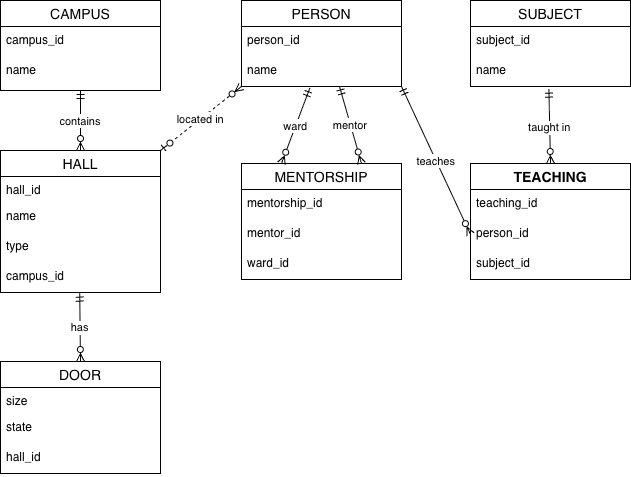
\includegraphics[width=0.7\textwidth]{Infological Model.png}
    \caption{Инфологическая модель}
\end{figure}

% ========== SECTION 5 ==========
\section{Даталогическая модель}

\begin{figure}[h]
    \centering
    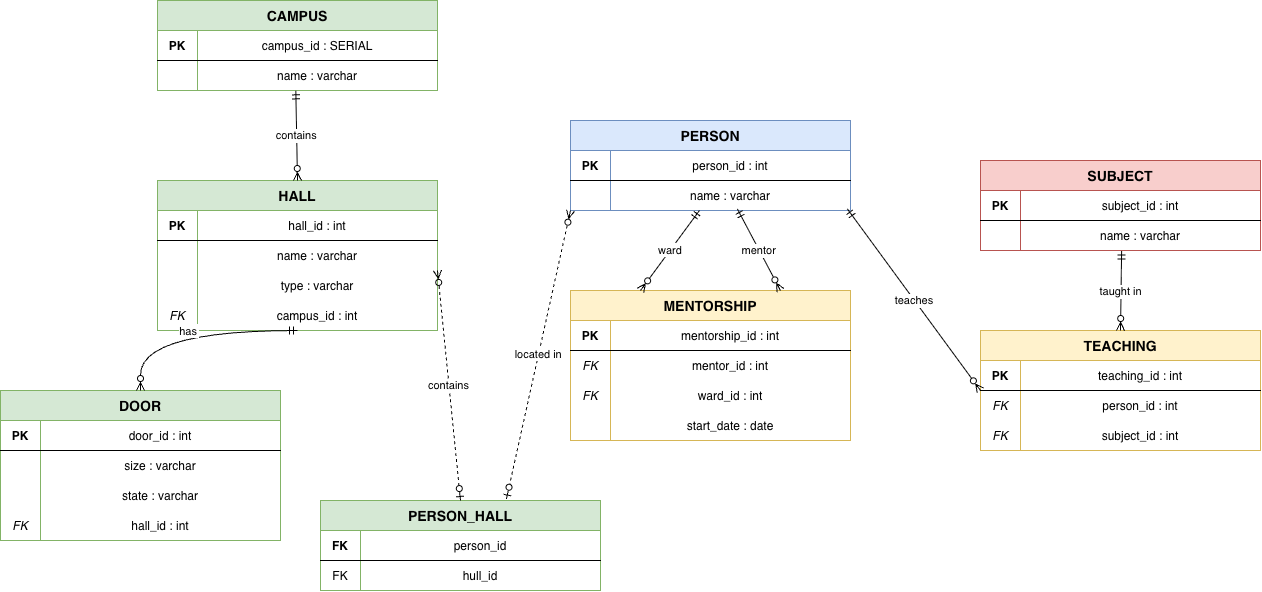
\includegraphics[width=0.7\textwidth]{Datalogical:Logical Model.png}
    \caption{Даталогическая модель}
\end{figure}
\newpage
% ========== SECTION 6 ==========
\section{Реализация даталогической модели на SQL}


\lstset{
    language=SQL,
    basicstyle=\ttfamily\scriptsize,
    keywordstyle=\color{blue},
    commentstyle=\color{gray},
    stringstyle=\color{red},
    breaklines=true,
    breakatwhitespace=true,
    columns=fullflexible,
    keepspaces=true,
    showstringspaces=false,
    frame=single,
    inputencoding=utf8
}


\begin{minted}[fontsize=\scriptsize, breaklines, linenos]{sql}

BEGIN;

CREATE TABLE person (
    person_id SERIAL        PRIMARY KEY,
    name      VARCHAR(100)  NOT NULL
        CONSTRAINT person_name_not_empty CHECK (TRIM(name) <> '')
);

CREATE TABLE campus (
    campus_id SERIAL        PRIMARY KEY,
    name      VARCHAR(100)  NOT NULL
        CONSTRAINT campus_name_not_empty CHECK (TRIM(name) <> '')
);

CREATE TABLE hall (
    hall_id   SERIAL        PRIMARY KEY,
    name      VARCHAR(100)  NOT NULL
        CONSTRAINT hall_name_not_empty CHECK (TRIM(name) <> ''),
    type      VARCHAR(50),
    campus_id INTEGER       NOT NULL
        REFERENCES campus(campus_id) ON DELETE CASCADE ON UPDATE CASCADE
);

CREATE TABLE door (
    door_id SERIAL        PRIMARY KEY,
    size    VARCHAR(50)   NOT NULL
        CONSTRAINT door_size_not_empty CHECK (TRIM(size) <> ''),
    state   VARCHAR(10)   NOT NULL
        CONSTRAINT door_state_valid CHECK (state IN ('open', 'closed')),
    hall_id INTEGER       NOT NULL
        REFERENCES hall(hall_id) ON DELETE CASCADE ON UPDATE CASCADE
);

CREATE TABLE subject (
    subject_id SERIAL        PRIMARY KEY,
    name       VARCHAR(100)  NOT NULL
        CONSTRAINT subject_name_not_empty CHECK (TRIM(name) <> '')
);

CREATE TABLE mentorship (
    mentorship_id SERIAL   PRIMARY KEY,
    mentor_id     INTEGER  NOT NULL
        REFERENCES person(person_id) ON DELETE CASCADE ON UPDATE CASCADE,
    ward_id       INTEGER  NOT NULL
        REFERENCES person(person_id) ON DELETE CASCADE ON UPDATE CASCADE,
    start_date    DATE     DEFAULT CURRENT_DATE,
    CONSTRAINT mentorship_no_self_ref CHECK (mentor_id <> ward_id),
    CONSTRAINT mentorship_unique_pair UNIQUE (mentor_id, ward_id)
);

CREATE TABLE teaching (
    teaching_id SERIAL   PRIMARY KEY,
    person_id   INTEGER  NOT NULL
        REFERENCES person(person_id)   ON DELETE CASCADE ON UPDATE CASCADE,
    subject_id  INTEGER  NOT NULL
        REFERENCES subject(subject_id) ON DELETE CASCADE ON UPDATE CASCADE,
    CONSTRAINT teaching_unique_pair UNIQUE (person_id, subject_id)
);

CREATE TABLE person_hall (
    person_id INTEGER  NOT NULL
        REFERENCES person(person_id) ON DELETE CASCADE ON UPDATE CASCADE,
    hall_id   INTEGER  NOT NULL
        REFERENCES hall(hall_id)     ON DELETE CASCADE ON UPDATE CASCADE,
    CONSTRAINT person_hall_pk PRIMARY KEY (person_id, hall_id)
);

CREATE INDEX idx_hall_campus       ON hall(campus_id);
CREATE INDEX idx_door_hall         ON door(hall_id);
CREATE INDEX idx_mentorship_mentor ON mentorship(mentor_id);
CREATE INDEX idx_mentorship_ward   ON mentorship(ward_id);
CREATE INDEX idx_teaching_person   ON teaching(person_id);
CREATE INDEX idx_teaching_subject  ON teaching(subject_id);
CREATE INDEX idx_person_hall_hall  ON person_hall(hall_id);

INSERT INTO person (person_id, name) VALUES
    (1, 'Коновалов Арсений Антонович'),
    (2, 'Клименков Сергей Викторович'),
    (3, 'Рыбинская Злата Владиславовна'),
    (4, 'Зайцева Ирина Сергеевна'),
    (5, 'Бобрусь Александр Владимирович');

INSERT INTO campus (campus_id, name) VALUES
    (1, 'Кронверкский проспект, 49'),
    (2, 'Ломоносова, 9');

INSERT INTO hall (hall_id, name, type, campus_id) VALUES
    (1, 'Большой актовый зал',              'актовый',       1),
    (2, 'Зал заседаний учёного совета',     'конференц-зал', 1),
    (3, 'Аудитория 325',                    'лекционный',    2),
    (4, 'Аудитория 101',                    'лекционный',    2);

INSERT INTO door (door_id, size, state, hall_id) VALUES
    (1, 'огромные', 'closed', 1),
    (2, 'огромные', 'open',   1),
    (3, 'средние',  'closed', 2),
    (4, 'малые',  'open',   3),
    (5, 'средние',  'closed', 4);

INSERT INTO subject (subject_id, name) VALUES
    (1, 'Базы данных'),
    (2, 'Математический анализ'),
    (3, 'Философия'),
    (4, 'Программная инженерия');

INSERT INTO mentorship (mentorship_id, mentor_id, ward_id, start_date) VALUES
    (1, 2, 1, '2024-09-01'),
    (2, 3, 4, '2024-09-01'),
    (3, 3, 5, '2024-02-01');

INSERT INTO teaching (teaching_id, person_id, subject_id) VALUES
    (1, 2, 1),
    (2, 2, 3),
    (3, 3, 2),
    (4, 3, 4),
    (5, 4, 3);

INSERT INTO person_hall (person_id, hall_id) VALUES
    (1, 1),
    (2, 1),
    (3, 2),
    (4, 3),
    (5, 4);

COMMIT;
\end{minted}

% ========== SECTION 7 ==========
\section{Вывод}

При выполнении лабораторной работы я познакомился с принципом проектирования «Top~--~Down», научился составлять инфологическую и даталогическую модель сущностей, по которым реализовал базу данных с помощью SQL.

\end{document}
